\documentclass[11pt, letterpaper]{article}
\usepackage[utf8]{inputenc}
\usepackage[margin=1in]{geometry}
\usepackage{enumitem}
\usepackage{indentfirst}
\usepackage{titling}
\usepackage{graphicx}
\usepackage{amsmath}
\usepackage{mathtools}
\usepackage{hyperref}
\graphicspath{ {./} }
\DeclareMathAlphabet{\altmathcal}{OMS}{cmsy}{m}{n}

\setlength{\parindent}{0cm}
\setlength{\parskip}{1em}
\renewcommand{\baselinestretch}{1.5}

\hypersetup{
    colorlinks=true,
    linkcolor=cyan,
    filecolor=magenta,      
    urlcolor=blue,
}

\title{Chapter II: Coulomb's Law}
\author{Chenyi Zhu}
\date{Jan 13th, 2020}

\begin{document}


\begin{titlingpage}
	\maketitle
		\begin{center}
				"Electricity is really just organized lightening." - George Carlin
		\end{center}
		
		\begin{figure}[h!]
			\centering
			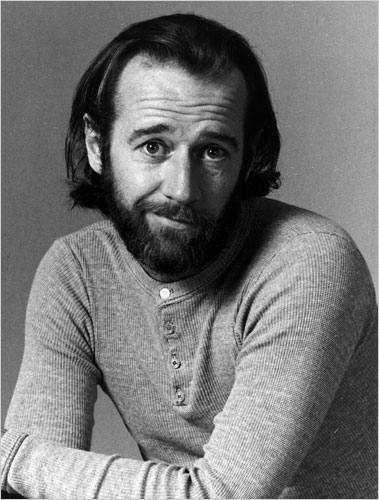
\includegraphics[scale=0.6]{george-carlin}
			\label{fig:comedian}
		\end{figure}
		
\end{titlingpage}
	
\section{Electric Charge, Coulomb's Law, and Superposition.} 

%\begin{itemize}[leftmargin=*, listparindent=0.7cm]

	%\item {\large Electric Charge} \par
	\subsection{Electric Charge}
	Introducing constant, the magnitude of the charge of an electron: \[|e^-| = 1.602 \times 10^{-19}
	\,C\] 
	\textbf{Note}: The \textbf{TOTAL} electric charge of an isolated system is conserved.
	
	\subsection{Coulomb's Law}
	Now we look at Coulomb's law, which defines the electric force as:
	\begin{equation}\label{eqn:coulomb-foce}
		\boxed{\vec{F} = k_e\frac{q_1q_2}{r^2}\,\hat{r} \qquad 
		k_e = \frac{1}{4\pi\varepsilon_0} = 8.9875 \times 10^9 \,N\cdot m^2/C^2}
	\end{equation}
	where $r$ is the distance between two particles and $k_e$ the Coulomb's constant. Bonus
	points for knowing \textbf{permittivity of free space}: \[\varepsilon_0 = 8.85 \times 
	10^{-12} \,C^2 / N\cdot m^2\] This will be useful later on when we work with capacitors. 

	\subsection{Superposition Principle}
	Working with electric forces is as simple as just adding \& subtracting vectors. Tip for solving
	problems that involve a set of charges $n$ and asks for the force an a particular particle j: using
	superposition principle: \[\vec{F_j} = \displaystyle\sum_{i = 1}^{n} \vec{F}_{i \neq j, j}\] and 
	remember, this is a sum of vectors, not scalar values!
%\end{itemize}


\newpage
\section{Electric Field.}

	\subsection{Electric Field}
	The electrostatic force, just like gravitational force, is able to act on an object from a distance 
	($r^2$) even if the objects are not touching each other. To explain this phenomenon, we say 
	that one charge creates a field in space which acts on other charges.

	While the charge $+Q$ creates a field everywhere in space, its strength varies. To quantify the
	strength of the field created by the point charge, we propose a test particle with infinitesimal 
	positive charge $+q$, and measure the force it experiences (hypothetically). The electric field is 
	defined as:
	\begin{equation}\label{eqn:electric-field}
		\boxed{\vec{E} \equiv \displaystyle\lim_{q \to 0} \frac{\vec{F}_e}{q} =\frac{1}{4\pi
		\varepsilon_0}\frac{Q}{r^2}\,\hat{r}}
	\end{equation}
	
	\begin{figure}[h!]
		\centering
		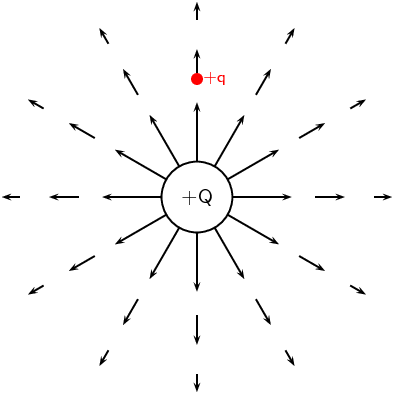
\includegraphics[scale=0.3]{point-charge}
		\caption{\href{https://intl.siyavula.com/read/science/grade-11/electrostatics/09
		-electrostatics-03}{Test charge $+q$ in field produced by $+Q$}.}
		\label{fig:point-charge}
	\end{figure}
	\noindent and we say (based on field theory) that charge Q produces an electric field $\vec{E}$ 		which exerts a force $\vec{F_e} = q\vec{E}$ on q.

	\noindent\textbf{Note}: we take $q$ to be infinitesimally small so that the field created by our 			test charge q does not interfere with the ``source charge'' Q.

	If we have a group of source charges $q_i$, the total electric field is the vector sum of the fields 
	of individual charges. \[\vec{E}_{total} = \displaystyle\sum_{i}\vec{E_i} = \displaystyle\sum_{i}
	\frac{1}{4\pi\varepsilon_0}\frac{q_i}{r^2}\,\hat{r}\]

\newpage
	\subsection{Electric Field Lines}
	For positive source charges, the electric field lines point outwards from the point charge, while
	for negative source charges the electric field lines point inwards to the point charge. Here, three
	scenarios are presented:

	\begin{figure}[h!]
		\centering
		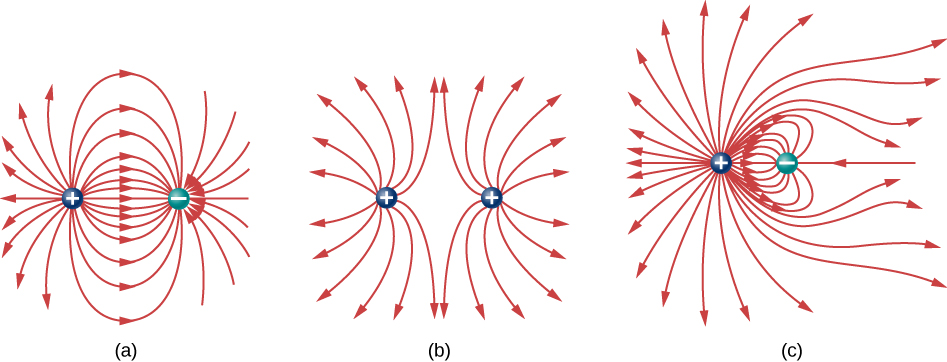
\includegraphics[scale=0.6]{three-scenarios}
		\caption{\href{https://tinyurl.com/v7fu6vm}{Three possible scenarios of fields' interaction.}}
		\label{fig:field-lines}
	\end{figure}

	In (a), we see two point charge sources of opposite signs and the field line created from this 
	interaction, and we call the pair an \textbf{electric dipole}. We can also tell immediately that 
	the two charges are of the same magnitude because they have the same field line density 
	(same number of field lines). In contrast, we observe in (c) that the positive charge is of 
	much higher magnitude than the negative charge, causing the field lines to concentrate 
	closer to the positive charge and producing a stronger field. 
	
	\subsection{Summary}
	\renewcommand{\theenumi}{\Roman{enumi}}
	\begin{enumerate}
		\item The direction of the electric field vector $\vec{E}$ at a point is tangent to the field lines. 
		\item The number of lines per unit area through a surface perpendicular to the line is 
				 devised to be proportional to the magnitude of the electric field in a given region. 
		\item The field lines must begin on positive charges (or ad infinitum) and then terminate on
				 negative charges (or ad inifinitum). 
		\item The number of lines that originate from a positive charge or terminating on a negative
				 charge must be proportional to the magnitude of the charge.
		\item Field lines CANNOT cross each other; otherwise the field would be pointing in two
				 different directions at the same point.
	\end{enumerate}
	
\section{Electric Dipole.}
	
	\subsection{Dipole}
	
	\begin{figure}[h!]
		\centering
		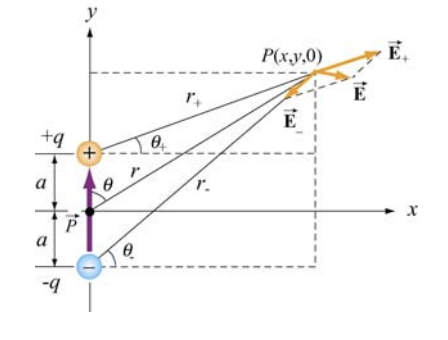
\includegraphics[scale=0.7]{dipole}
		\caption{The electric dipole.}
		\label{fig:dipole}
	\end{figure}
	
	As mentioned in the previous section, an electric dipole consists of two equal but opposite 
	charges. Say we have two point charges $+q$ and $-q$ along the $y$-axis, separated by a 
	distance $d$. Then the dipole moment vector $\vec{p}$ points from $-q$ to $+q$ is:
	\begin{equation}\label{eqn:dipole}
		\boxed{\vec{p} = 2aq\,\hat{j}}
	\end{equation}
	where the magnitude of the vector is $p = 2qa$, $q > 0$. For a system of $N$ charges, the
	overall electric dipole vector is defined as:
		\[\vec{p} \equiv \displaystyle\sum_{i = 1}^{N} q_i\vec{r}_i\]
	where $\vec{r}_i$ is the position vector of charge $q_i$.
	
	\subsection{Electric Field of a Dipole}
	\begin{figure}[h!]
		\centering
		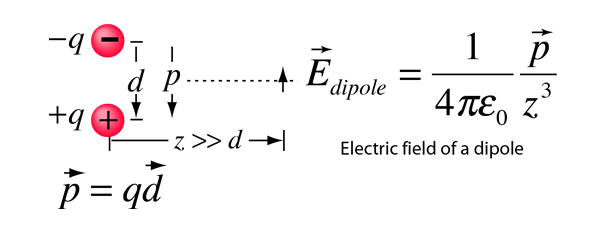
\includegraphics[scale=1.3]{dipole-field}
		\caption{\href{http://hyperphysics.phy-astr.gsu.edu/hbase/electric/dipole.html}{Electric
		field of a dipole.}}
		\label{fig:dipole-field}
	\end{figure}
	\noindent\textbf{Note}: The distance between $+q$ and $-q$ is MUCH smaller than the dipole's 
	distance to the test charge.

\section{Charge Densities.}

So far we have only seen point charges and, at most, a dipole. The electric fields due to these are
fairly straightforward to compute with the superposition principle, but what if we encounter a large
number of charges distributed (not necessarily evenly) in some region in space? Here we introduce
the novel concept of \textbf{charge density}. This will come up a lot in problems!

\begin{figure}[h!]
	\centering
	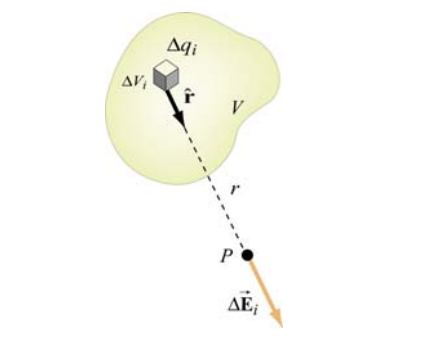
\includegraphics[scale=0.65]{volume}
	\caption{Electric field due to small charge element $\Delta q_i$ at $P$.}
\end{figure}
	\subsection{Volume Charge Density}
	Let's find the electric field at point P. Consider small volume element $\Delta V_i$ and the small,
	corresponding charge element $\Delta q_i$. Assume the distances among between the charges
	within $\Delta V_i$ is MUCH smaller compared to the distance from $\Delta V_i$ to point $P$
	(which is $r$ in our case). Make $\Delta V_i$ to be infinitesimally small and obtain:
	\begin{equation}\label{eqn:volume-charge-density}
		\boxed{\rho(\vec{r}) = \lim_{\Delta V_i \to 0} \frac{\Delta q_i}{\Delta V_i} = \frac{dq}{dV}}
	\end{equation}
	where the dimension of $\rho(\vec{r})$ is charge/unit volume $(C/m^3)$. To find the total
	charge of the volume $V$:
		\[Q = \displaystyle\sum_{i} \Delta q_i = \displaystyle\iiint_{V} \rho(\vec{r}) \,dV\]
	\noindent\textbf{Note}: $\rho(\vec{r})$ is analogous to mass density $\rho_m(\vec{r})$ we
	have seen before, given a large number of atoms are densely packed within a volume $V$:
		\[M = \iiint_{V} \rho_m(\vec{r}) \,dV\]
	
	\subsection{Surface Charge Density}
	Now that we got volume over with, the rest are fairly standard. If we have charge spread out
	across a surface $S$ of area $A$ with a surface charge density $\sigma$:
	\begin{equation}\label{eqn:surface-charge-density}
		\boxed{\sigma(\vec{r}) = \frac{dq}{dA}}
	\end{equation}
	where $\sigma(\vec{r})$ has units charge/unit area $(C/m^2)$. Total charge over surface:
		\[Q = \displaystyle\iint_S\sigma(\vec{r}) \,dA\]
	
	\subsection{Line Charge Density}
	Moving on to the simplest one-dimensional geometry, a line. Suppose we have a certain amount
	of charge distributed across a line of length $l$, then the linear charge density $\lambda$ is:
	\begin{equation}\label{eqn:linear-charge-density}
		\boxed{\lambda(\vec{r}) = \frac{dq}{dl}}
	\end{equation}
	where $\lambda(\vec{r})$ has units charge/unit length $(C/m)$. To obtain the total charge of 
	the line, do:
		 \[Q = \displaystyle\int_{line}\lambda(\vec{r}) \,dl\]
	
	\noindent\textbf{Note}: if the charge is uniformly distributed throughout the geometry, then the 
	charge densities $(\lambda, \sigma, \rho)$ become uniform as well (otherwise you may end up 
	with step functions depending on your charge density).
	
	\subsection{Continuous Charge Distributions}
	If we take a small charge element $dq$, its electric field according to Coulomb's law would be:
		\[d\vec{E} = \frac{1}{4\pi\varepsilon_0}\frac{dq}{r^2}\,\hat{r}\]	
	and therefore, all you have to do to find the electric field $\vec{E}$ at a point $P$ is to integrate
	$\frac{dq}{r^2}\,\hat{r}$. Do your conversion of $dq$ based on the charge density formulae 
	(charge densities are typically given in any problem, or the derivation will be straightforward),
	and also convert $r^2$ and $\hat{r}$ to standard Cartesian units of $\hat{x}, \hat{y}, and\hat{z}$
	if necessary (remember that it is not always easy to work these problems out in Cartesian 
	coordinates, in which case it would be easiest to keep $r$ as it is).
	
	\subsection{General Strategies}
	
	\renewcommand{\theenumi}{\Roman{enumi}}
	\begin{enumerate}
	
	\item You should first draw out the direction of the vector and note its magnitude. If we have a
	symmetric shape, think about whether the vectors can cancel in some way, which will 
	save you a massive amount of computation and time.
	
	\item Start with $d\vec{E} = \frac{1}{4\pi\varepsilon_0}\frac{dq}{r^2}\,\hat{r}$
	\item Rewrite $dq$ and plug back into $d\vec{E}$:
		\begin{equation}		
			dq= \begin{cases}
				\lambda\,dl \quad \text{(length)}\\
    				\sigma\,dA \quad \text{(area)}\\
    				\rho\,dV \quad \text{(volume)}\\
			 \end{cases}
		\end{equation}
	\item Choose one of the following coordinate systems, whichever suits the problem:
	\begin{figure}[h!]
		\centering
		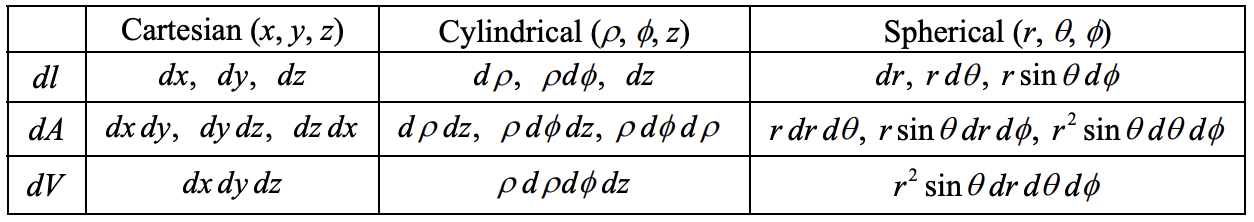
\includegraphics[scale=0.7]{coordinates}
		\caption{Coordinate systems.}
		\label{fig:coordinates}
	\end{figure}
	\item Rewrite $d\vec{E}$ in terms of the chosen coordinate system and integrate.
	\end{enumerate}
	
	\newpage
	\subsection{Examples}
	\begin{figure}[h!]
		\centering
		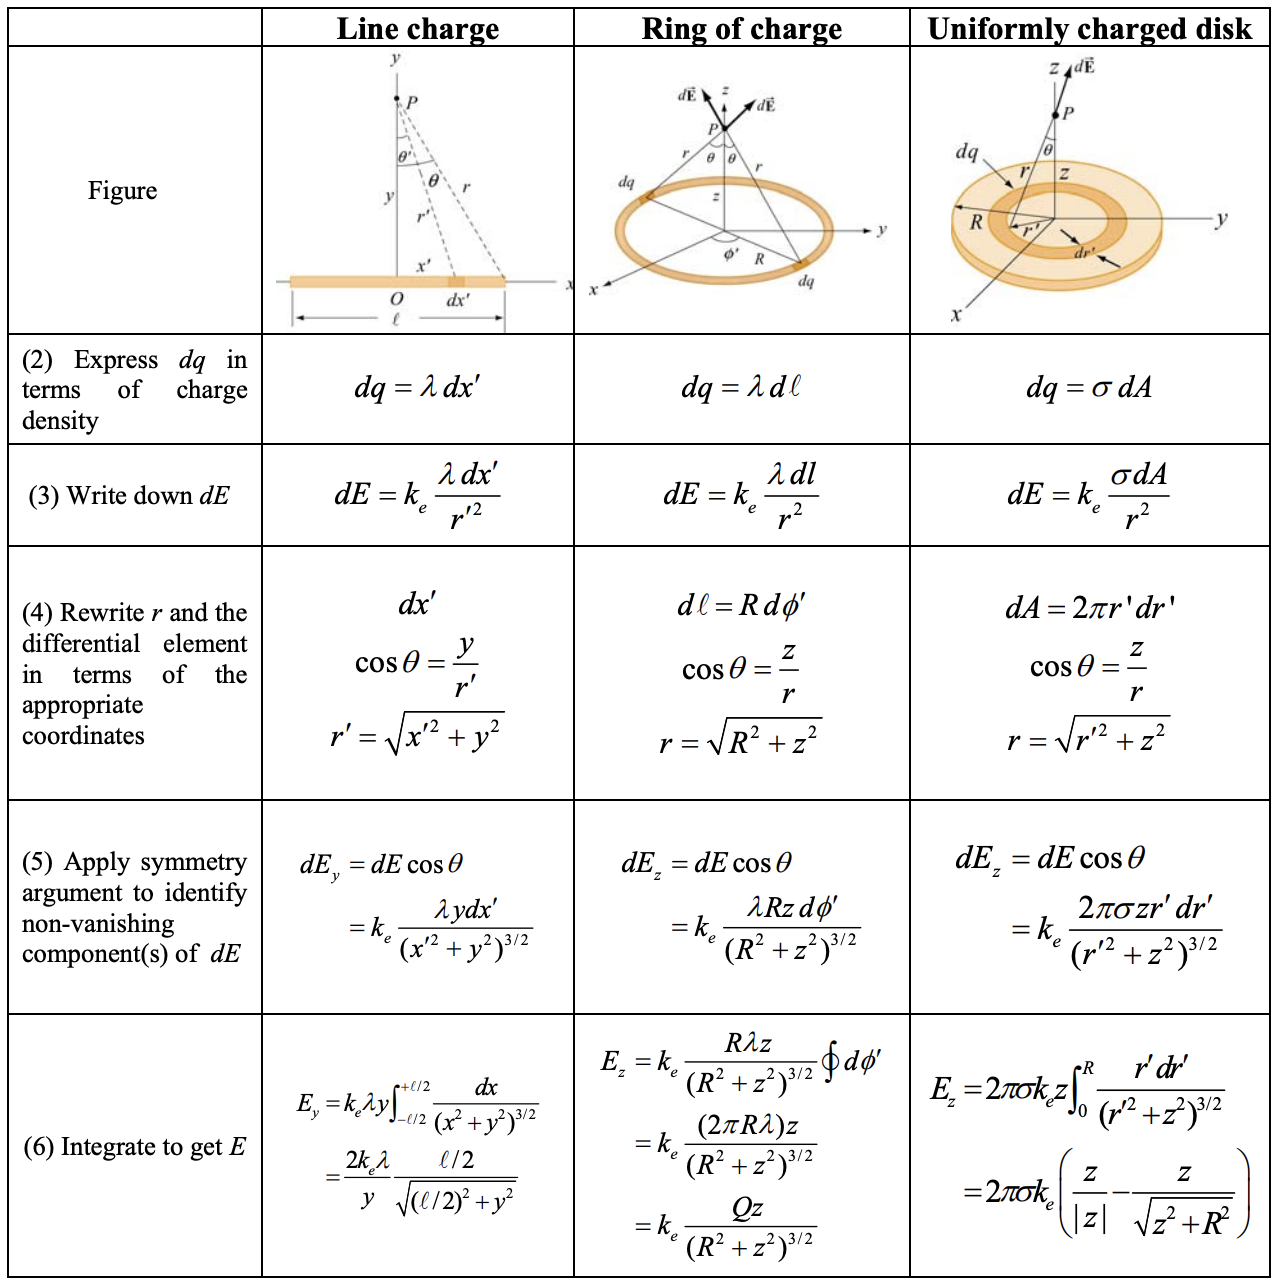
\includegraphics[scale=0.7]{charge-density}
		\caption{Most common examples.}
		\label{fig:examples}
	\end{figure}
	
	\noindent\textbf{Note}: Remember your kinematic equations! There may be questions that
	involve an object subject to the influence of both the gravitational AND electrostatic forces.
	Look \href{https://en.wikipedia.org/wiki/List_of_equations_in_classical_mechanics}{here} for
	a comprehensive list.
	\newpage
\setlength{\parindent}{0.0cm}
\section{Exercises.}
\subsection{Electric Forces}
%3.1
\textbf{Problem 1}: Calculate the ratio of the electrostatic to gravitational interaction forces 
between two electrons, or two protons. At what value of $\frac{q}{m}$ would the two forces
be equal?

%3.4
\textbf{Problem 2}: Two positive charges $q_1$ and $q_2$ are located at the points
with radial vectors $\vec{r}_1$ and $\vec{r}_2$. Find a negative charge $q_3$ and a radial 
vector $\vec{r}_3$ of the point at which it has to be placed for the force acting on each of 
the three charges to be $0$.

%3.11
\textbf{Problem 3}: A system consists of a thin charged wire ring of radius $R$ and a long
uniformly charged thread oriented along the axis of the ring, with one of its ends coinciding 
with the center of the ring. The total charge of the ring is $q$, and the charge density of the
thread if $\lambda$. Find the interaction force between the ring and the thread.

\subsection{Electric Fields}
%3.8
\textbf{Problem 4}: A thin half-ring of radius $R$ is uniformly charged with a total charge $q$. 
Find the electric field at the curvature center of this half-ring.

%3.15
\textbf{Problem 5}: A thread carrying a uniform charge density $\lambda$ has configurations 
shown in Figure 8 a) and b). Assuming the curvature radius $R$ to be considerably less than
the length of the thread, find the electric field at the point $O$.
\begin{figure}[h!]
	\centering
	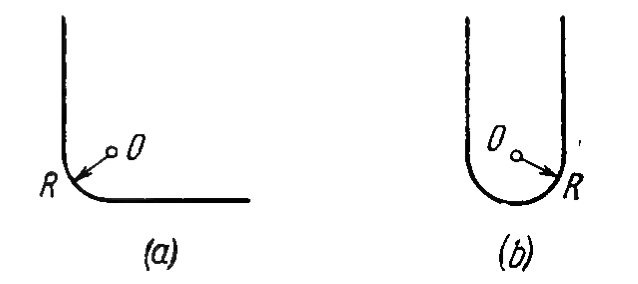
\includegraphics[scale=0.6]{irodov_3-15}
\end{figure}

%3.16
\textbf{Problem 6}: A sphere of radius $r$ carries a surface charge of density $\sigma=ar$,
where $a$ is a constant vector and $r$ the radius vector of a point on the sphere relative to 
its center. Find the electric field at the center of the sphere.

\end{document}
